\documentclass{MScthesisITEM}

% this package is just to generate text for demo-purposes
\usepackage{blindtext}

%Packages added by Dean
\usepackage{multirow}

\title{Title} % The title of your assignement; NB use \newlinetitle to start a newline
\author{Firstname Lastname} % Your firstname and lastname
\professor{Firstname Lastname, Affiliation} % Affiliation = ITEM for instance
\supervisor{Firstname Lastname, Affiliation}

%% Uncomment the following in case you want subfigures; note that there will be a warning for the caption package
% \let\subcaption\undefined
% \let\subfloat\undefined
% \usepackage[bf]{caption}
% \usepackage{subcaption}

\DeclareGraphicsExtensions{.pdf,.jpg}
\graphicspath{{./figs/}}

\loadglsentries{glossary}
\makeglossaries

\begin{document}
\selectlanguage{english}
\pagenumbering{roman}
\pagestyle{plain}

%% Only for the project
\titleITEM

%% Only for the master's thesis; for the project report the description is taken from It's Learning and added by the department
% \selectlanguage{english} % Change to 'norsk' if you are writing in Norwegian
% \begin{titlingpage}

\noindent
\begin{tabular}{@{}p{4cm}l}
\textbf{Title:} 	& \thetitle \\
\textbf{Student:}	& \theauthor \\
\end{tabular}

\vspace{4ex}
\noindent\textbf{Problem description:}
\vspace{2ex}

\noindent \Blindtext[2][1]
\vspace{6ex}

\noindent
\begin{tabular}{@{}p{4cm}l}
\textbf{Responsible professor:} 	& \theprofessor \\
\textbf{Supervisor:}			& \thesupervisor \\
\end{tabular}

\end{titlingpage}
% \cleardoublepage

%% There must be an abstract in English, even though the main text is in Norwegian
\selectlanguage{english}
\pagestyle{empty}
\begin{abstract}
  \noindent
Recent studies have shown that only 1 in 5 Norwegian adults and elderly reach the national goal of 30 minutes of activity each day. Increasing the activity of the elderly is one of the main foci of Hagen Utvalget, a committee appointed by the Norwegian government to solve future challenges in care service. The report emphasizes on using technology to help solve such health problems. Using a sensor called the activPAL we are able to classify a patients activity into periods spent walking, standing and sitting/laying. Data gathered by the sensor is used to create visualizations illustrating the patients activity throughout a week. The question we aim to answer is: Which visualizations are most fitting to aid physiotherapists in interpreting and understanding accelerometer data in communication with patients and other healthcare workers? A prototype was created and reviewed in two focus groups with physiotherapists working for Trondheim Kommune. The process was iterative and feedback from the first focus group was used to modify and improve the prototype before the second focus group. In addition to the prototype, scenarios for the use of the system and a set of functional and user experience requirements were created. All of the participants were positive to the prototype presented and could see themselves using such a system in their work. The participants were also convinced that using such technology would improve the quality and effectiveness of their work.
\end{abstract}

\cleardoublepage

%% Only for the master's thesis; if the main text is in English and you can write Norwegian, there must be an abstract in Norwegian as well.A
% \selectlanguage{norsk}
% \renewcommand{\abstractname}{Sammendrag}
\begin{abstract}
\noindent
Studier har vist at bare én av fem voksne og eldre når den nasjonale anbefalingen om 30 minutters daglig aktivitet. Å øke aktiviteten hos de eldre var en av de viktigste utfordringene for Hagen Utvalget, et utvalg oppnevnt av regjeringen for å løse fremtidige utfordringer i omsorgstjenesten. Hagen Utvalgets rapport trekker frem viktigheten av å bruke ny teknologi for å løse disse utfordringene. Ved hjelp av en sensor kalt activPAL kan vi klassifisere pasienters aktivitet i tre ulike kategorier: gående, stående og stillesittende. Data samlet av sensoren brukes til å lage visualiseringer som illustrerer pasienters aktivitet gjennom en uke. Spørsmålet vi prøver å besvare er: Hvilke visualiseringer er best for å hjelpe fysioterapeuter med å tolke og forstå akselerometerdata fra pasienter, i kommunikasjon med pasienter og andre helsearbeidere? Det ble laget en prototype som ble vurdert i to fokusgrupper bestående av fysioterapeuter. Prosessen var iterativ og tilbakemeldinger fra den første fokusgruppen ble brukt til å modifisere og forbedre prototypen før den andre fokusgruppen. I tillegg til prototypen, ble scenarier for bruk av systemet og et sett av funksjonelle og brukeropplevelses krav opprettet. Kravene og prototypen danner anbefalinger for hvordan å lage visualiseringer som kan benyttes av fysioterapeuter til å løse spesifikke oppgaver. Alle deltakerne av fokusgruppene var positive til prototypen som ble presentert og kunne se for seg å bruke slik teknologi i sitt eget arbeid. Deltakerne var også overbevist om at bruk av slik teknologi vil øke kvaliteten og effektiviteten på deres arbeid.
\end{abstract}

% \cleardoublepage

\selectlanguage{english}% Change to 'norsk' if you are writing in Norwegian

\renewcommand{\abstractname}{Preface}
\begin{abstract}
\noindent
This master thesis is the final part required for us to attain a Master of Science degree at the Norwegian University of Science and Technology (NTNU). The work in this thesis was conducted from the start of February to the end of June 2013 at the Department of Computer and Information Science (IDI).

\noindent
We would like to thank our supervisor Professor Dag Svanæs for the invaluable guidance we have received during our work. We also wish to extend gratitude to the domain expert at St. Olav's Hospital and the physiotherapists who participated in the two focus groups. Without their knowledge and insight this project would not have been possible. 
\end{abstract}

\cleardoublepage

% similarly you may add a separate acknowledgments page

\tableofcontents*
\cleardoublepage

%% include if relevant
\listoffigures
\cleardoublepage

%% include if relevant
\listoftables
\cleardoublepage

%% include if relevant
\listofalgorithms
\addcontentsline{toc}{chapter}{List of Algorithms}
\cleardoublepage

%% include if relevant
\printglossary[title=List of Symbols, style=long]
\cleardoublepage
\glsaddall[]

%% include if relevant
\printglossary[title=List of Acronyms,type=\acronymtype] % prints just the list of acronyms
\cleardoublepage

\pagenumbering{arabic}
\pagestyle{ruled}
%% include here the other chapters
% Chapter 1

\chapter{Introduction} % Main chapter title
\label{chapter1} % For referencing the chapter elsewhere, use \ref{Chapter1} 

\section{Purpose/Motivation}
The elderly population is in a constant rise, currently 15\% of the Norwegian population is above the age of 65. By the turn of the century the elderly population is expected to double \cite{elder}. The initial rise of the elder population will be most noticeable in those below the age of 80, as seen in figure \ref{fig:elderPopulation}. After 2025 a great increase in the population above the age of 80 is expected. The Norwegian Institute of Public Health* reports that two out of three above the age of 75 consider themselves having ``good health'' but only a third preserve this level of health until death \cite{elder}.

\begin{figure}[h!]
	\centering	
		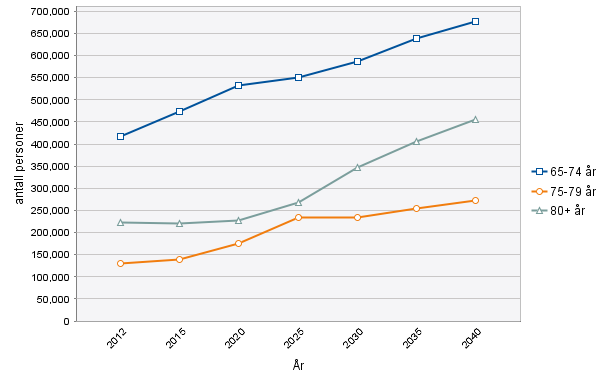
\includegraphics[width=0.5\textwidth]{eldrevekst.png}
		\caption{\footnotesize Elder population estimation \cite{elder}}
		\label{fig:elderPopulation}
\end{figure}
In 2010 one of the largest ever systematic efforts to describe the global health situation was conducted. The article was later published in The Lancet \cite{globalBurden}. One of their many findings was that since 1970 men and women have gained an additional ten years to their life expectancy, but spend more time living with injuries and illness. %KOMMER TILBAKE HIT

In the late 1990s the Norwegian statistical bureau* published a paper predicting a major increase in the elderly population \cite{eldreEksplosjon}. The working population compared to the retired currently holds a ratio of 5 to 1. This is expected to drop below 3 by the year 2040. Because of this, the greatest challenges within welfare are expected to occur between 1998 and 2020. 

With such predictions the Norwegian government formed a committee (referred to as Hagen-utvalget*) that would investigate the current situation and suggest solutions for accommodating the increase in the percentage of elderly \cite{haagen}. One of the conclusions in the report was that too little of today's technology is incorporated as welfare technology* for the elderly. A Danish report refereed to by Hagen-utvalget* states that around 20\% of the tasks performed by healthcare personnel could be completely or partly replaced by technology \cite{kmd}. 

To handle the rising percentage of elderly, Hagen-utvalget* suggest a national three step program that focuses on using welfare technology to diminish falls, social isolation and cognitive failure. Thus improving the overall quality of life for the elder population as well as reducing the workload for health care personnel. Step 3 states that:
\begin{quote}
\textit{``Opt on technology that stimulates, activates and structures daily life.''}
\end{quote}
One way of using modern technology to reduce sedentary behaviour can be to through self-reflection using personal informatics tools such as the activPAL. %Does this work, I feel it's a little out of place...

The amount of time adults spend in a sedentary position has increased over the last 30 years. The reasons for this are many, but increased use of technology and ease of transport are one of the main factors \cite{sedentaryBehaviour}. An American study shows that 1 of 4 US adults spend 70\% of their waking hours in a sedentary position, 30\% in light activity, and little to no time is spent exercising.

In the last decade research has started to emerge that links extended periods of sedentary time to metabolic risks\cite{sedentaryTime}, obesity, and abnormal glucose metabolism \cite{breaksSedentary}. It is suggested that prolonged periods of sedentary time should be avoided by increasing the number of breaks during sedentary time, and these findings suggest new public health recommendations \cite{breaksSedentary}. Another study goes as far as stating that prolonged sedentary time is strongly related to metabolic risks independent of physical activity \cite{sedentaryActivity}, and that older people benefit more from reducing the sedentary time. What has not been shown by research is how long a subject can stay sedentary before it has negative impact on the individuals health, or how long the breaks between sedentary time should be.

Personal Informatics* has become an emerging branch of technology to help individuals collect personal information for the purpose of self-reflection and self-monitoring. We will look relevant trends and technology later in this project. By using personal data and visualize their patterns we hope to bring awareness to their activity levels, and identify periods of long sedentary time. 

\section{Project context/Thesis Scope}
This project is a cooperation between the Department of Computer and Information Science (IDI)* at the Norwegian University of Science and Technology (NTNU) and St. Olavs University Hospital in Trondheim. The project...

\section{Research questions}

\section{Research method}

\section{Thesis outline}

\chapter{Technology} % Main chapter title

\label{chapter2} % For referencing the chapter elsewhere, use \ref{Chapter1} 


\section{HTML5}
HTML is a markup language for the creation of web pages. HTML describes the structure and the contents of the web page. In later years, the need for advanced styling and complex interaction with web pages has made CSS and JavaScript increasingly popular. HTML5 was created as a response to this, HTML5 is an umbrella term for creating web pages using HTML5, CSS3 and JavaScript.

HTML5 has simplified the syntax compared to earlier versions. New tags have been added to better represent the modern web page elements. Other features include media tags which greatly simplifies adding multimedia content, such as playing audio and video files. More importantly for our project is the extensive support for interactive and animated graphics through the \emph{canvas}- and \emph{svg}-tag.

The new features of HTML5 and CSS3 make it much easier to create web applications for multiple platforms and screen sizes. After the smartphone and tablet revolution creating responsive and adaptable websites has become more important. The new features included in HTML5 give large amount of flexibility with respect to the user interface and graphical visualizations.

%Is this section too short? On the other hand, is there anything more to write about CSS3 in this context?
\section{CSS3}
\emph{Cascading Style Sheets} (CSS) is a language used to describe the styling of an HTML document. Using CSS the size, color and look of HTML elements can be configured. A new feature in CSS3, which is part of HTML5, is \emph{Media Queries}. With Media Queries it is possible to specify different styling relative to the size of the screen. This functionality is useful when creating applications that target devices with different screen sizes, such as smartphones, tablets and laptops. 

%Is this section to short? Is it too stripped?
\section{JavaScript}
JavaScript is the main scripting language for web pages. It is a client-side scripting language that allows programmers to add functionality to otherwise static HTML-pages. While CSS3 takes care of the styling of HTML-elements, JavaScript is used to create customized behaviour. All modern browsers have JavaScript engines/interpreters that compile and run JavaScript code.

JavaScript is now an industry standard maintained by ECMA International. The standardized version of the script is named ECMAScript. Today ECMAScript and JavaScript are used interchangeably, and JavaScript is often used to refer to ECMAScript. Because different browsers have different implementations of the JavaScript engine, slight variations in the way JavaScript code will run on these browsers exists.

Together with HTML5 and CSS3, JavaScript is great for creating web applications that can be designed to run on both mobile and stationary devices. JavaScript has a multitude of useful open source libraries that can be used to create complex user interaction, animation, and custom graphics.

\section{Data-Driven Documents}
One of the challenges in this project is to create different visualizations to represent the activity patterns of subject. Creating custom graphics in HTML5 can be done using both the canvas- and the svg-tag. In this project SVG is used. Scalable Vector Graphics (SVG) is an image format that uses XML encoding. All popular browsers, and most mobile devices, support rendering of the svg-tags.

Creating graphics using svg-tags directly is cumbersome and time consuming. Therefore a framework that greatly simplifies this task is used. \emph{Data-Driven Documents} (D3) is an open source framework written in JavaScript. D3 supports animation and interaction with the SVG elements. This allows us to explore if animation and interactivity can improve the readability of the visualizations.

\section{activPAL}
To record the activity pattern of elderly a device called \emph{activPAL} will be used. activPAL has the shape of a small rectangle and is worn on the thigh. When the device is active it continuously records accelerometer data using an internal accelerometer. This data can be interpreted using a algorithms provided by PAL Technologies.

When the activity data has been gathered the \emph{Intelligent Activity Classification}-algorithm, provided by PAL Technologies, is used to classify the data into three different types of behaviour: sitting/laying, standing and walking. Because activPAL is worn on the thigh the accelerometer is unable to detect the difference between sitting and lying. Number of steps is also counted when walking. This data can be used to calculate how fast the person was walking.

%Is this section too short and a little strange? Maybe it should be moved to the end of the section?
Several studies have concluded that the activPAL is viable for recording and classifying activity \cite{grant2006, ryan2006, grant2008, tsavourelou}. activPAL has also been used in multiple studies for obtaining and analysing activity patterns \cite{grant2010, lord, ryan2010}.

Though this projects main focus is how to present the data and not analysis of it, the accuracy is not a huge concern. It is however important that the data presented to test subjects* reflects a realistic activity pattern. Another important factor is to show that data from a simple monitoring device can be used to create complex visualizations.

\chapter{Related Products and Research} % Main chapter title

\label{chapter3} % For referencing the chapter elsewhere, use \ref{Chapter1} 

Self-monitoring through technology is still in it's early stages, some view it as a temporary interest that will fade over time, others look at this technology as an invaluable tool to help understand ourselves better. There is no denying that research, communities, and products have surfaced that aim to understand and provide help with self-monitoring. In this section we will start out by looking at the communities around the technology, and look at some of the existing products. Finally we will present earlier research done that is relevant to our thesis.

\section{Communities}
Currently there are two names that stand out within self-monitoring: Quantified Self, and Personal Informatics. Quantified self is a community of end users who share data and exchange experiences with tools that help them collect information. Personal Informatics on the other hand is academic and developer driven, they desire to understand what makes a good tool, and how the user interacts with such technology.

\subsection{Quantified Self}
In 2011 a movement known as Quantified Self*\cite{quantifiedSelf} had their first conference \cite{bodyHackers}, here people shared data that they had collected about themselves width different types of devices. The goal is to gather as much information about yourself as possible, to learn about yourself through quantitative data. Members of Quantified Self* collect information about everything from sleep patterns and diets to mood and stress levels.

%Is this better?
To promote further development in tools that gather these types of information, the participants of Quantified Self has worked closely with companies and individuals that create personal informatics tools. Devices such as Nike's FuelBand \cite{fuelBand} and Fitbit \cite{fitBit} are results of this cooperation, and both products have been well received.

%Maybe make it clearer that it is an exchange of information between QS and developers?
%The exchange of information within the movement between users and tool makers %Tool makers, really?
% allows for new, exciting and relevant technology to be developed. The FuelBand\cite{fuelBand}, Fitbit\cite{fitBit} are some of results of this cooperation, and both products seem to be well received by the movement.
 
\subsection{Personal Informatics}
Personal informatics is the label used to classify tools that help people collect personal information for the purpose of self-monitoring and self reflection. These tools are used to help individuals gain self-knowledge about their behaviour, habits, and thoughts\cite{personalInformatics}.

The Computer-Human Interaction (CHI) conference has since 2010 \cite{chi2010} held workshops and accepted papers on Personal Informatics. The aim is to increase understanding of how the tools affect the user, explore new possibilities, and overall improvement of the user experience.
	
\section{Products}
%Maybe something should be added here?
\subsection{Nike+}
The Nike+ concept has existed since 2010 and is the brand name Nike uses for sports related activity tracking. A sensor in the shoe and a receiver connected to an iPod was the first Nike+ product. Since then the Nike+ line has expanded into Kinect Games, sport watches and shoe implants \cite{nikeProducts}. As the product line increased so did the community around it. Every Nike+ device now requires an online profile where user can store information, create goals, and look at their history. However the Nike+ FuelBand \cite{fuelBand} is the first product aimed at monitoring the user outside of their workout, and motivating them to reach the daily activity goals.

FuelBand was released in early 2012 and was the first commercial wrist worn activity monitor. The wristband contains a 3-axis accelerometer that tracks the users wrist movement. Recorded activity is converted to \emph{Nikefuel} \cite{nikefuel}, NikeFuel is a unit of measurement used by all Nike activity trackers, however there are no details on how activity is converted to NikeFuel, as the algorithm is proprietary. The wristband does calculate steps and calories burned, but the NikeFuel is the prime focus of their product line. NikeFuel does not take into account gender, height, weight, but looks purely at activity. Meaning that a mile will award the same amount of points to users of very different physiology. The daily progress is represented through a ring that fills up when the FuelBand detects activity, the ring is full once the daily activity goal is reached. If the NikeFuel goal is exceeded by a certain percentage the ring will gain visual improvements. 

NEED IMAGE FROM REVIEW HERE! DO WE NEED APPROVAL!?%IMAGE HERE IF THEY GET APPROVED BY SVANÆS

The information from the FuelBand can be uploaded to an iPhone or laptop which then send the information to the Nike+ servers and update the users profile. The online profile provides detailed information of the users activity, showing steps, calories burned, active time, distance travelled and average fuel. Charts can be displayed for weeks, months or years. This allows the user to track their progress and look at how often they achieve or go way above their goals.\cite{fuelbandTechSpce}. 
 
NEED IMAGE FROM REVIEW HERE! DO WE NEED APPROVAL!?%SHOW ACTIVITY BREAKDOWN
 
Virtual trophies are awarded for various achievements such as gathering an X amount of NikeFuel or beating the set goal by a 100\%. These trophies can then be shared with friends or displayed on the public profile to show off achievements. The FuelBand can display simple information such as how far the user is from his daily goal, steps taken, and calories burned. A review has reported that the NikeFuel concept can almost become an addiction and lead to doing some last minute workouts in order to reach the goal \cite{fuelbandDcRain}.

%I agree that this might be a little too specific, since we are not using this technology.  %Unsure if specific technical details should be mentioned, such as that it communicates through bluetooth etc. I figure the relevancy of these products is more on how they do things and what we can learn.

\subsection{Fitbit}
The Fitbit concept wishes to be much more involved in the subjects daily life. While the Nike+ only tracks activity, Fitbit lets the user log their sleep, food, heart rate, blood pressure and glucose. It does not specifically target exercises, but instead allows the user to track their everyday life. The product line currently consists of the Zip, One, and Aria. The Zip and One are hip worn activity trackers and will automatically update the users online profile when synced. The automatic activity trackers count only steps, but other activities and even manual labour are supported and can be entered by the user. Fitbit One is also able to track stairs climbed, hours slept and sleep quality allowing this to be automatically tracked. Aria is the Fitbit scale, if the device is linked to an online profile it will automatically update BMI, Weight, and body fat percentage at each weighing. Currently there are no official Fitbit devices that track blood pressure, heart rate or calorie intake, these all have to be entered manually if the user wishes to do so. There is also a journal where the user can create entries to describe their day and rate their mood.

Similar to the Nike+ the Fitbit allows the user to set daily goals, but as the Fitbit does not use the NikeFuel system, it enables the user to set 3 separate goals: steps taken, floors climbed, and calories burned. The Fitbit does provide an active score, but there is no emphasis on it. A daily activity breakdown is provided, this breaks the activity levels for the day into 4 categories: sedentary, lightly active, fairly active, and very active. All the goal histories can be viewed on the online profile and can be categorized into day, week, months and years. This is also applicable to other measurements such sleep, mood, blood pressure and glucose levels. 

NEED IMAGE FROM REVIEW HERE! DO WE NEED APPROVAL!?

As goals are reached Fitbit members are awarded badges. These badges are very similar to the Trophies that Nike+ awards their users. It can either be for having a very active day or lifetime achievements such as accumulating over 50,000 steps. The user can choose if he wishes these badges to be public or personal, and can be displayed on the profile if desired.

The Flex is the first wrist worn activity monitor from Fitbit, and is slated for release in June 2013. It will have the same functionality as the Fitbit One, with the exception of an altimeter, meaning it can not measure stairs climbed. This is considered to be the greatest upcoming competitor for the Nike+ FuelBand.

%We should write about the many smartphone apps that offer self-tracking.
\section{Related Research}

%THIS SECTION NEEDS REVIEW!
\subsection{Stage-Based Model of Personal Informatics Systems}
When talking about personal informatics it is useful to divide the personal informatics system into stages. Ian Li et al. created a stage-based model (see figure~\ref{fig:stageModelPI}) \cite{li2010} with five different stages: \emph{preparation}, \emph{collection}, \emph{integration}, \emph{reflection}, \emph{action}. The preparation stage is the stage before actual data is collected. This stage describes how and why people are motivated to collect data about themselves, which data is to be collected, and how.Most elderly would not by them self be motivated to start collecting data about them selves. Healthcare personnel can be an important motivator in this regard, by explaining the concept and benefits of self-reflection. 

\begin{figure}[h!]
	\centering
		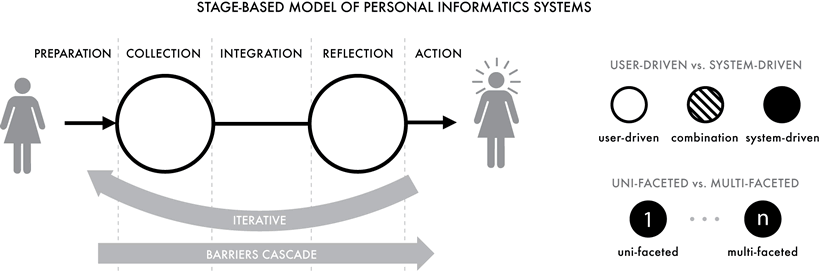
\includegraphics[width=0.5\textwidth]{stageModelPI.png}
		\caption{\footnotesize Taken from the Ian Li article \cite{li2010}}.
		\label{fig:stageModelPI}
\end{figure}

In the collection stage, data is collected. In this project all data collection was system driven, and the participants did not have to write down or be aware of their activity during this stage. Using a fully automated system will make it more attractive, since there is almost no effort connected to the collection of data. The sensor is small and barely noticeable.

The stage before reflection is the integration stage. This is the stage where the collected data is transformed into something that is useful. Creating visualizations is a powerful way to present large amount of data in a way that can be understood by humans in a short amount of time. 

In the reflection stage the users looks at the different charts to get an overview of the behavioural patters throughout the week. Since the data presented is collected over a longer period it is important that some time is used to analyse the data and identify patterns that may be instrumental in the last stage, action. Healthcare personnel can supervise the self-reflection and give explanations and instructions on how to interpret the different visualizations for best effect.

The last stage is the action stage. In this stage the user should change their behaviour to improve themselves. This stage is probably the most important, but also the hardest. For the users to improve they have to want to improve and they need to know how to improve. The reflection stage can help to identify periods of the day with long sedentary behaviour and with the help of the healthcare personnel a plan with concrete goals should be created. 

Ian Li et al. also identified a set of barriers for each of the five steps in the model. Barriers are problems that the participants of the study had when performing each step of the model. We will now list some of barriers that are applicable to our project, and how we aim to solve them. 

In the collection stage some of the most important barriers are having the right tools, remembering to collect data and lack of time. All of these barriers should be easily countered by the use of the activePAL sensor. Data is automatically recorded and the users does not have to do anything except wear the sensor and make sure not to break it while it is being uses. Using a fully system-driven approach in the collection stage give us more consistent and reliable data.

The integration stage is also mostly system-driven in our solution. The most important barriers for this step are related to transcribing and organizing data. Our program handles all the parsing and presents the data as different visualizations, so the transcribing will not be hard. Currently the application only handles a singe entry of data, and lets you see different visualizations of this data. Future work may be adding the possibility of comparing not only days, but weeks and months.

Notable barriers in the reflection stage are lack of time, visualizations, interpretation and self-criticism. Lack of time should not be to much of an issue for us, because the elderly population will most likely have more than enough time to participate in tests recommended to them by healthcare personnel. The visualization and interpretation barriers are central for our project. The goal of this project is to measure the effectiveness of different types of visualizations and discuss what types visualizations gives the most useful information as well as how easy they are to interpret. Self-criticism can also present a problem, some users may have a hard time looking at and reflecting over personal data. With the help and encouragement of healthcare personnel it is possible to minimize this problem. 

For the action stage it is critical that the users get motivated to change for the better, through reflecting on the data collected. It may also be helpful for the user to be provided with suggestions on how to improve their behavioural patterns. Tools could also be created to help remind the users to be more active, for example by adding reminders into calendars.

%This section is not written yet.
%Using this model Li %should I mention the others? Use et al.?
%came up with four recommendations for personal informatics systems. 
%\begin{quote}
%	Personal informatics systems should
%	1) be designed in a holistic manner across the stages.
%	2) allow iteration between stages.
%	3) apply an appropriate balance of automated technology and user control within each state to facilitate the user experience.
%	4) explore support for associating multiple facets of people's lives to enrich the value of the system.
%\end{quote}

\chapter{Methodology} % Main chapter title

\label{chapter4} % For referencing the chapter elsewhere, use \ref{Chapter1} 

\section{Background}
All research methods fall into two categories: Quantitative and qualitative research \cite{realWorldResearch}. Qualitative research is suitable when one wishes to gain an understanding of an underlying phenomenon through explanations and reactions the subjects bring forward. To achieve this the researches have to interview and observe the subjects who are evaluating the object. Quantitative research are appropriate when one wishes to gain a broader understanding of a phenomenon by seeing the effects of some manipulation or activity on the phenomenon. Unlike qualitative research, quantitative research focuses on measurement, quantification and generalization of data. This in turn promotes comparison and statistical analysis of the data gathered.



\section{Focus group}
Focus group, or group interview is an informal technique that can help software developers identify the users needs and feelings about the system in question. The technique can be used both before interface design and long after implementation. 

According to Nielsen \cite{focusGroup} the focus group should have at least six participant to maintain a flowing discussion and provide different perspectives. The participants should be representative of the intended users, or be the final users themselves. Sessions normally last two hours and are run by a moderator. The moderator is responsible for keeping the discussion relevant to the session goals while letting everyone contribute and not hindering the input of ideas and comments from the participants. %Liker ikke helt den siste setningen
A single session may not be representative enough or can get sidetracked, it is therefore important to run more than one focus group.

Nielsen \cite{focusGroup} discusses two pitfalls with focus groups: Sessions are in groups therefore the participants are unable to test the system themselves, so a demo is normally provided instead. The problem with such a demo is that the participants never have to question what to do next or consider the meaning of the screen options. The second problem is that what participants say they want is not necessarily what they need, or things described by the moderator might be perceived differently by the participants. By providing concrete examples through prototypes of the technology, one can minimize this problem.

\chapter{Prototype} % Main chapter title
Vi må vell kanskje rename denne seksjonen ,til graphs eller noe. Ettersom det er jo egentlig ikke prototypen som er i fokus
\label{chapter5} % For referencing the chapter elsewhere, use \ref{Chapter1} 

\section{Initial Graphs}
\label{sec:initialGraphs}

%We must settle on a name for these types of graphs
\subsection{Fractional charts}
These types of charts shows the sum of time spent sedentary, standing, and walking. Summing over the three classifications makes it easy to get an overview of the day as a whole. Though the summation gives a great overview, details are lost and it is not possible to pinpoint when each activity occurred during the day. (Name of chart)* can be useful for quickly identifying days with a low amount of activity, before spending time looking at more detailed visualisations. It might also serve as an alert for subjects with a low activity level.

\subsubsection{Pie chart}
The pie chart is a standard way of showing fraction of time spent on each behavioural pattern. The overall design of the pie chart is very standard. We decided to create a separate legend instead of writing a descriptive text on different pie slices. The legend is a simple box which connects a behavioural pattern to each colour. The exact percentage for each behavioural pattern is also displayed.

\subsubsection{Symbolic}
Another approach is to remove the legend and instead use illustrations so that the user intuitively understands what each colour or box corresponds to. Since the illustrations are had to fit into a pie slice this chart uses scaled boxes instead of a circle to represent the fraction. 

The first idea was to only use the illustrations \ref{fig:symbolicPie}, without the boxes, and scale the height to represent the ratio between each activity classification. However this idea was discarded because it was too hard to identify the ratio between the different illustrations. This is much easier with boxes.

%We may have to redraw this picture compared to the explanation in this section?
\begin{figure}[h!]
	\centering
		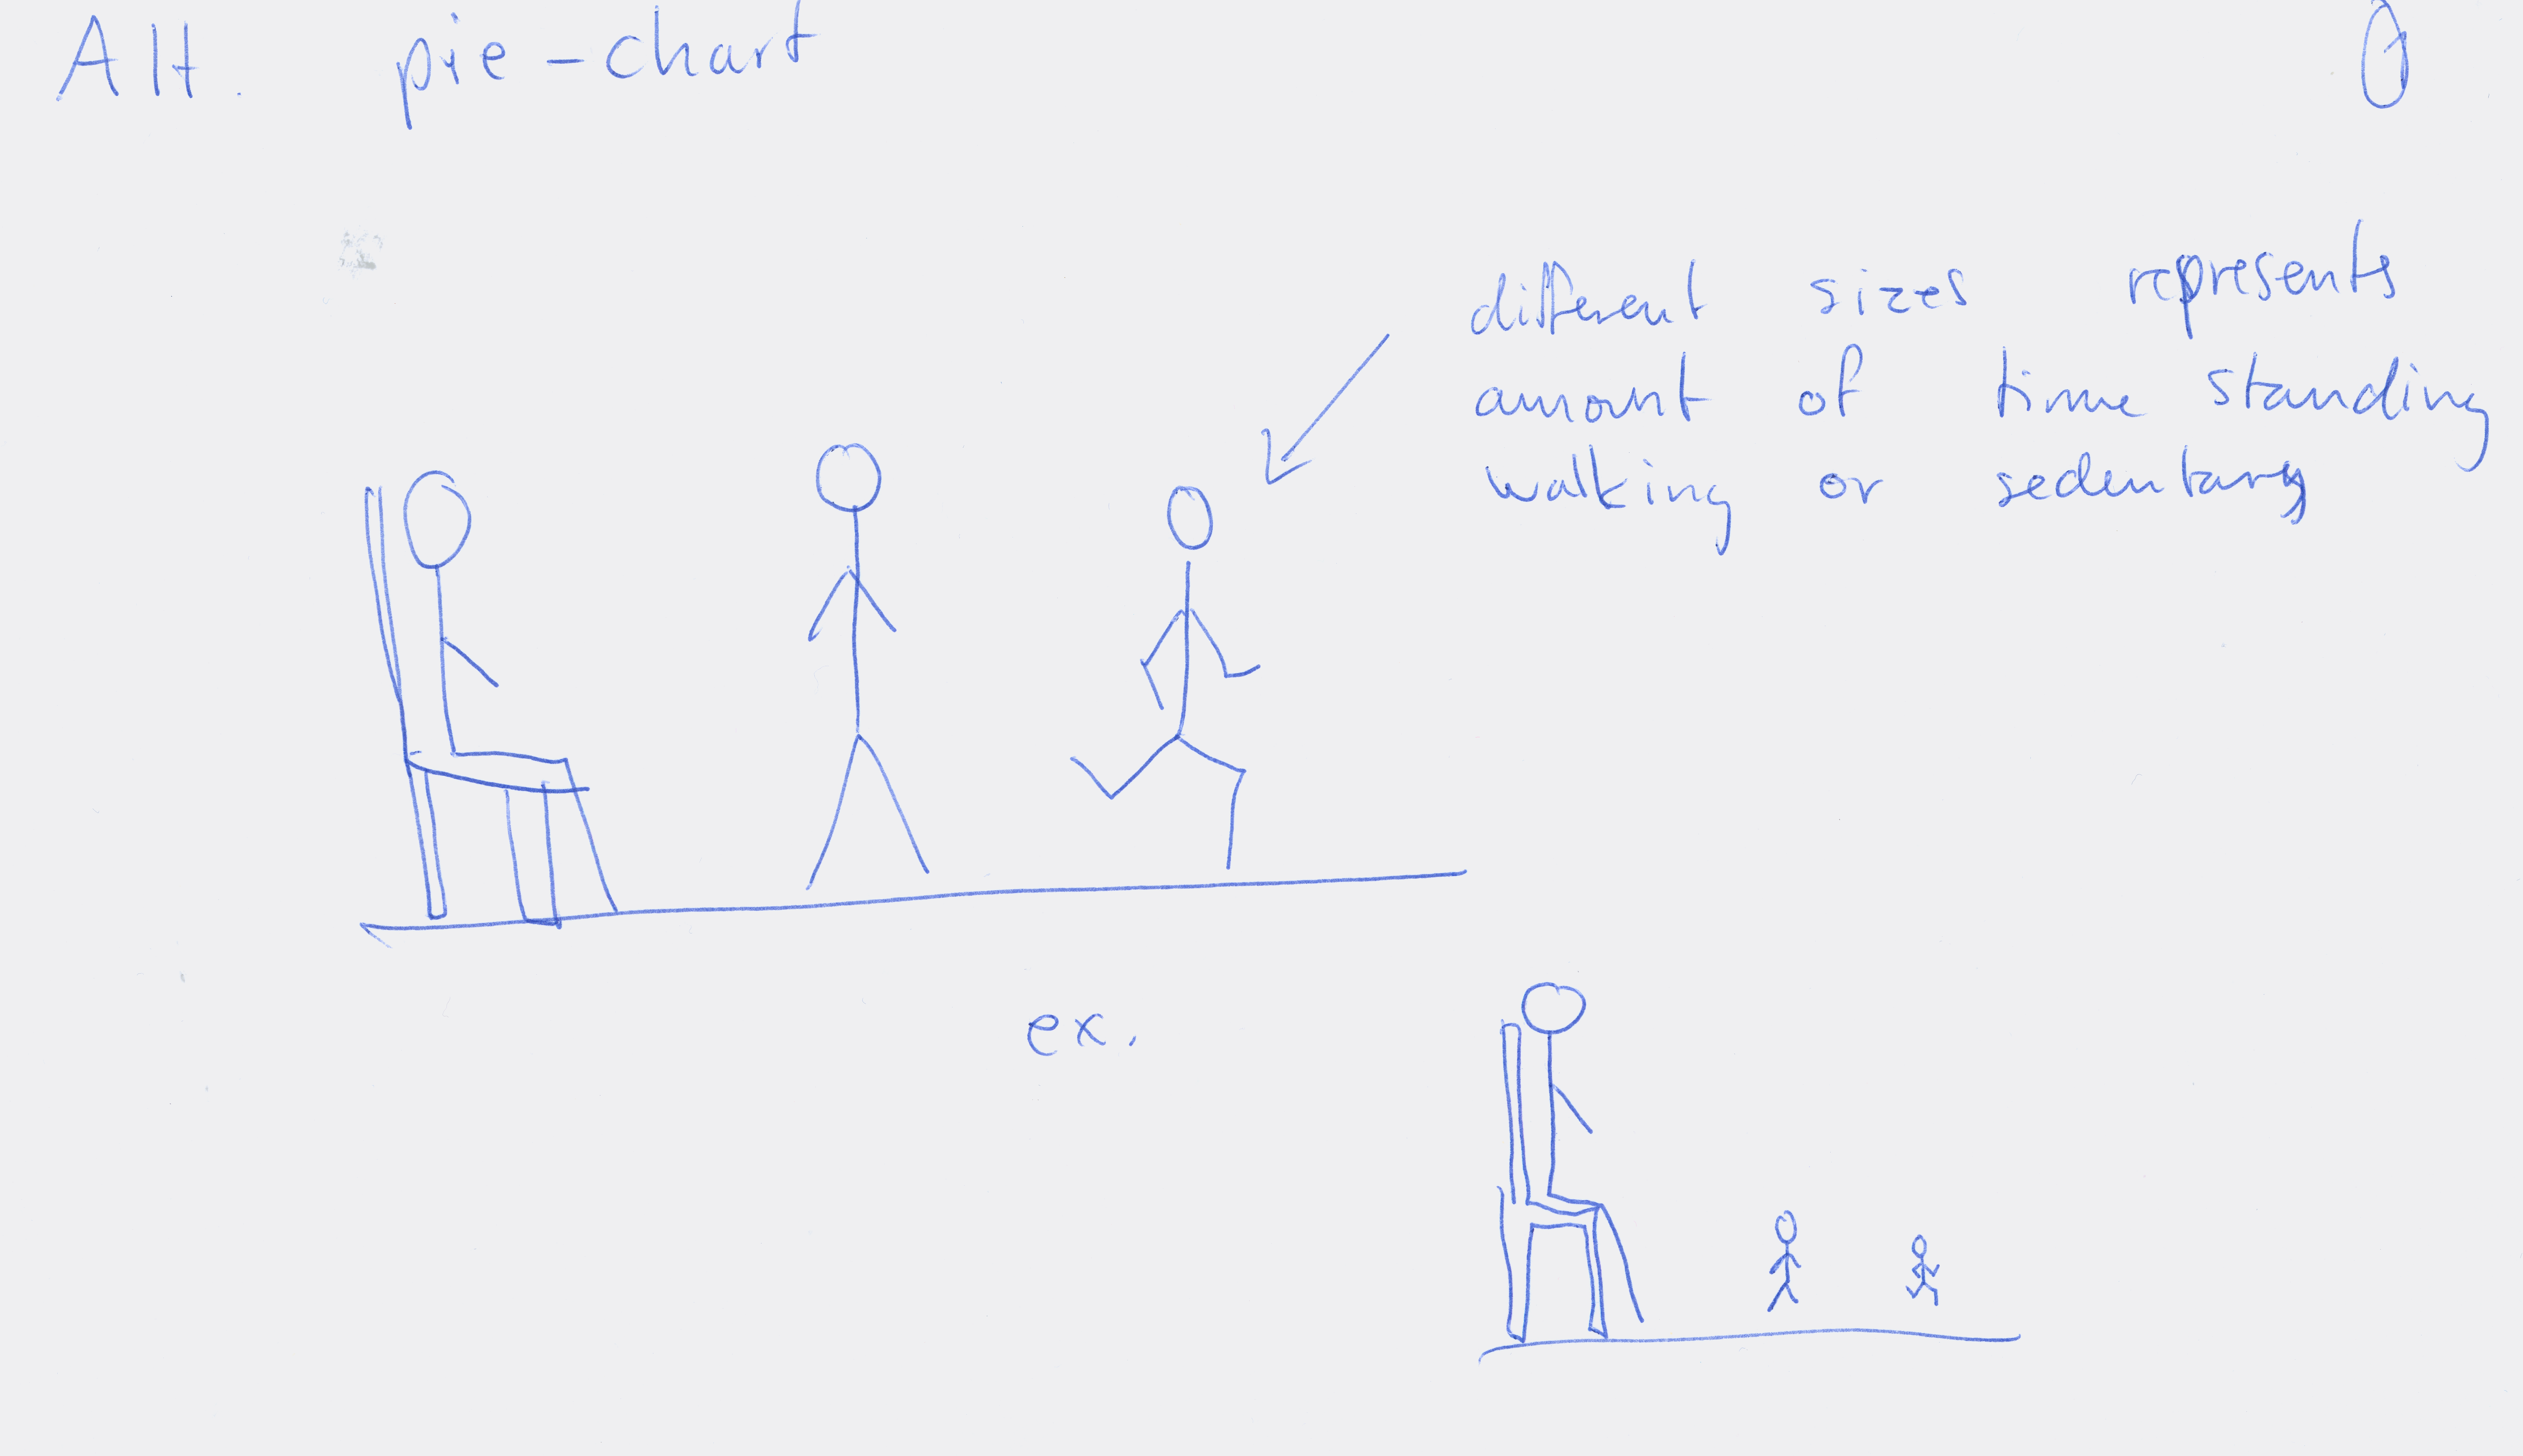
\includegraphics[width=0.7\textwidth]{stickSketch.png}
		\caption{\footnotesize Rough drafts of a symbolic "pie chart"}
		\label{fig:symbolicPie}
\end{figure}

\subsubsection{Ball chart}
Another approach, is to include some more details into a pie chart style, by using balls instead of normal pie slices. Each ball represents an interval of one of the classifications, so that many balls of one colour both represents the amount of that behaviour and shows how long each period of that behaviour was. Figure %need a figure here
shows an example of such a graph. The benefit with this type of graph is that you easily can identify if you have long stretches of sedentary behaviour. Taking small breaks with active behaviour can help ``split up'' those balls, which may be beneficial for your health. Adding interactivity to the chart you can select each ball and see what time it corresponds to. This way you can quickly find the larger balls and identify what time of the day this behaviour occurred. 
%I don't even know man, fuck you.

\subsection{Timeline}
Timeline visualisations are effective at illustrating when various activities occurred during the day. The illustration uses a long horizontal bar that has different colours for different behavioural classification. Such a bar can be used to identify points during the day where the subject is in a sedentary position for too long. By looking at multiple days, the user can detect patterns in the day where he needs to be more active.

\subsubsection{Continuous}
One approach to this visualization is to create a continuous timeline that contains every little detail of behaviour, see figure \ref{fig:timelineContinuous}. The continuous timeline is useful for quickly identifying periods of the day with unsatisfactory behaviour, but the detail can also be distracting and make it harder to read the graph. Adding a fourth colour to highlight long periods of sedentary behaviour can make the timeline easier to interpret.

%Perhaps represent the block based one instead?
\begin{figure}[h!]
	\centering
		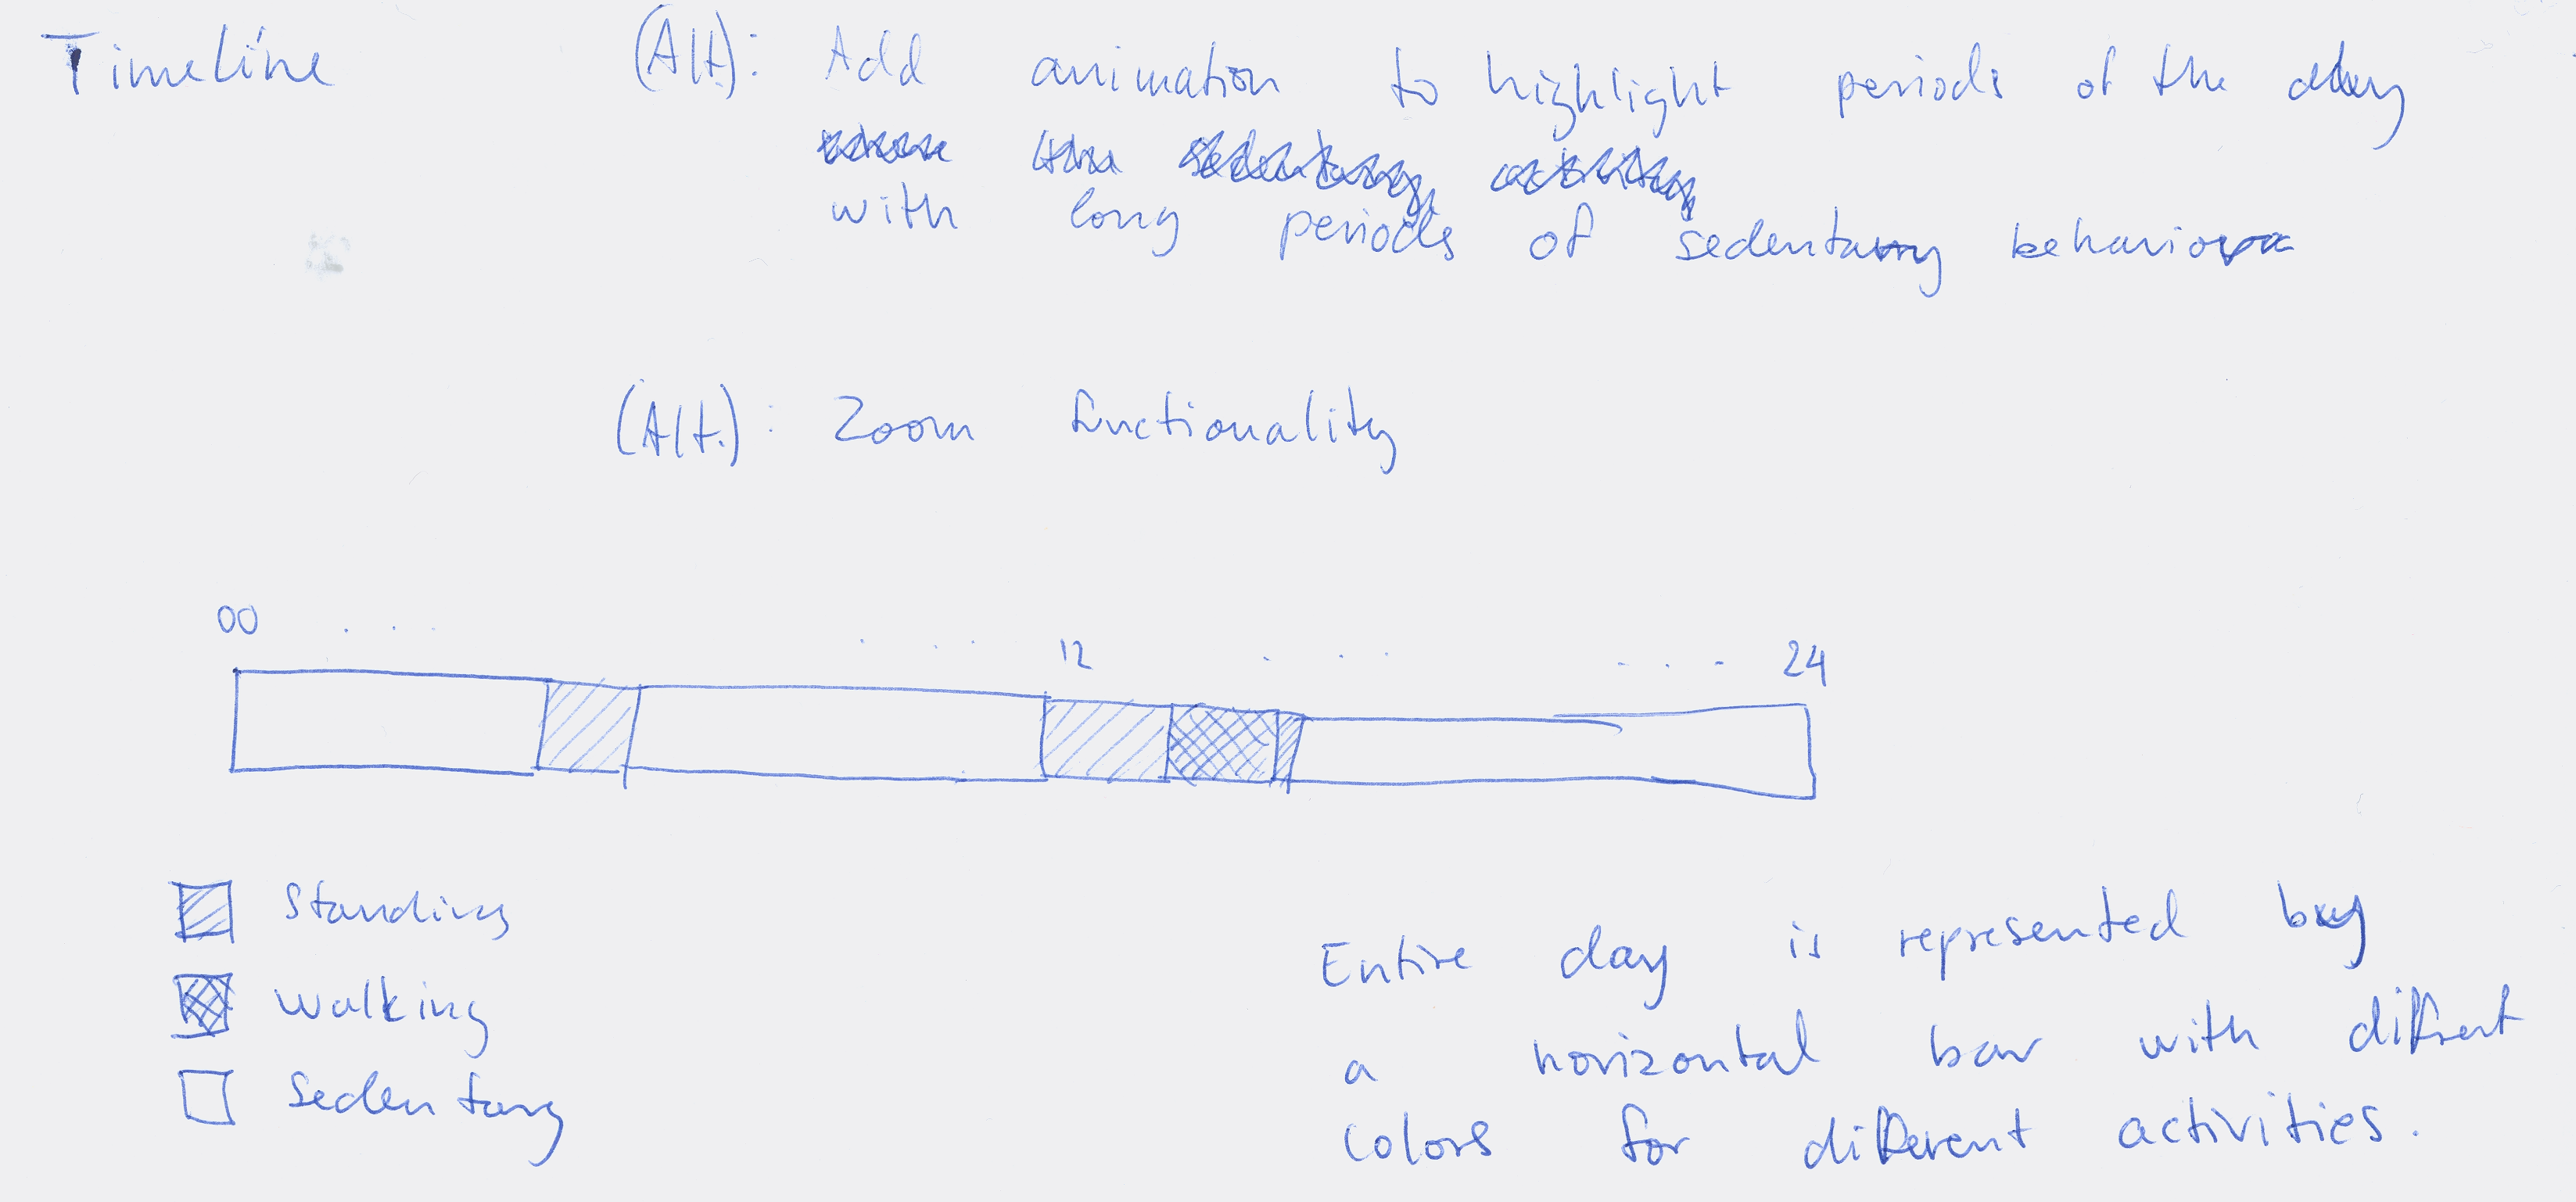
\includegraphics[width=0.7\textwidth]{continousTimelineSketch.png}
		\caption{\footnotesize Timeline with hour blocks}
		\label{fig:timelineContinuous}
\end{figure}
%Does this part need more of an introduction?
%Why would you make it less formal?
%Skrevet det litt om for å gjøre det mindre formelt
We came up with a suggestions to represent the passing of time during a day by using an animated timeline and stick figures. The timeline will be drawn in real time while stick figures simultaneously perform the corresponding activities. By displaying the day gradually we hope that the subject will gain a firm understanding of their day. This means that this visualization can not be used to gain a quick overview, but is intended to be used when viewing a day for the first time.

The more motivational approach would be to replace the stick figure with an analogy or metaphor. Instead of a stick figure, a flower could be used. Activity would allow the plant to get sunlight, making it grow. Sedentary positions would make the weather cloudy and the flower would be unaffected.

\subsubsection{Blocks}
Instead of having a continuous scale, a blocked approach can be used, as seen in figure \ref{fig:timelineBlocks}. The timeline would be divided into 24 blocks, each block corresponding to an hour. A gradient colour scale would be used to represent the amount of activity inside the hour block. This should make it easy to identify hours in the day where prolonged sedentary positions are present. Giving feedback about specific hours might make it easier to interpret and make use of the chart, because you are alerted to certain hours of the day where you should be more active.

%Perhaps represent the block based one instead?
\begin{figure}[h!]
	\centering
		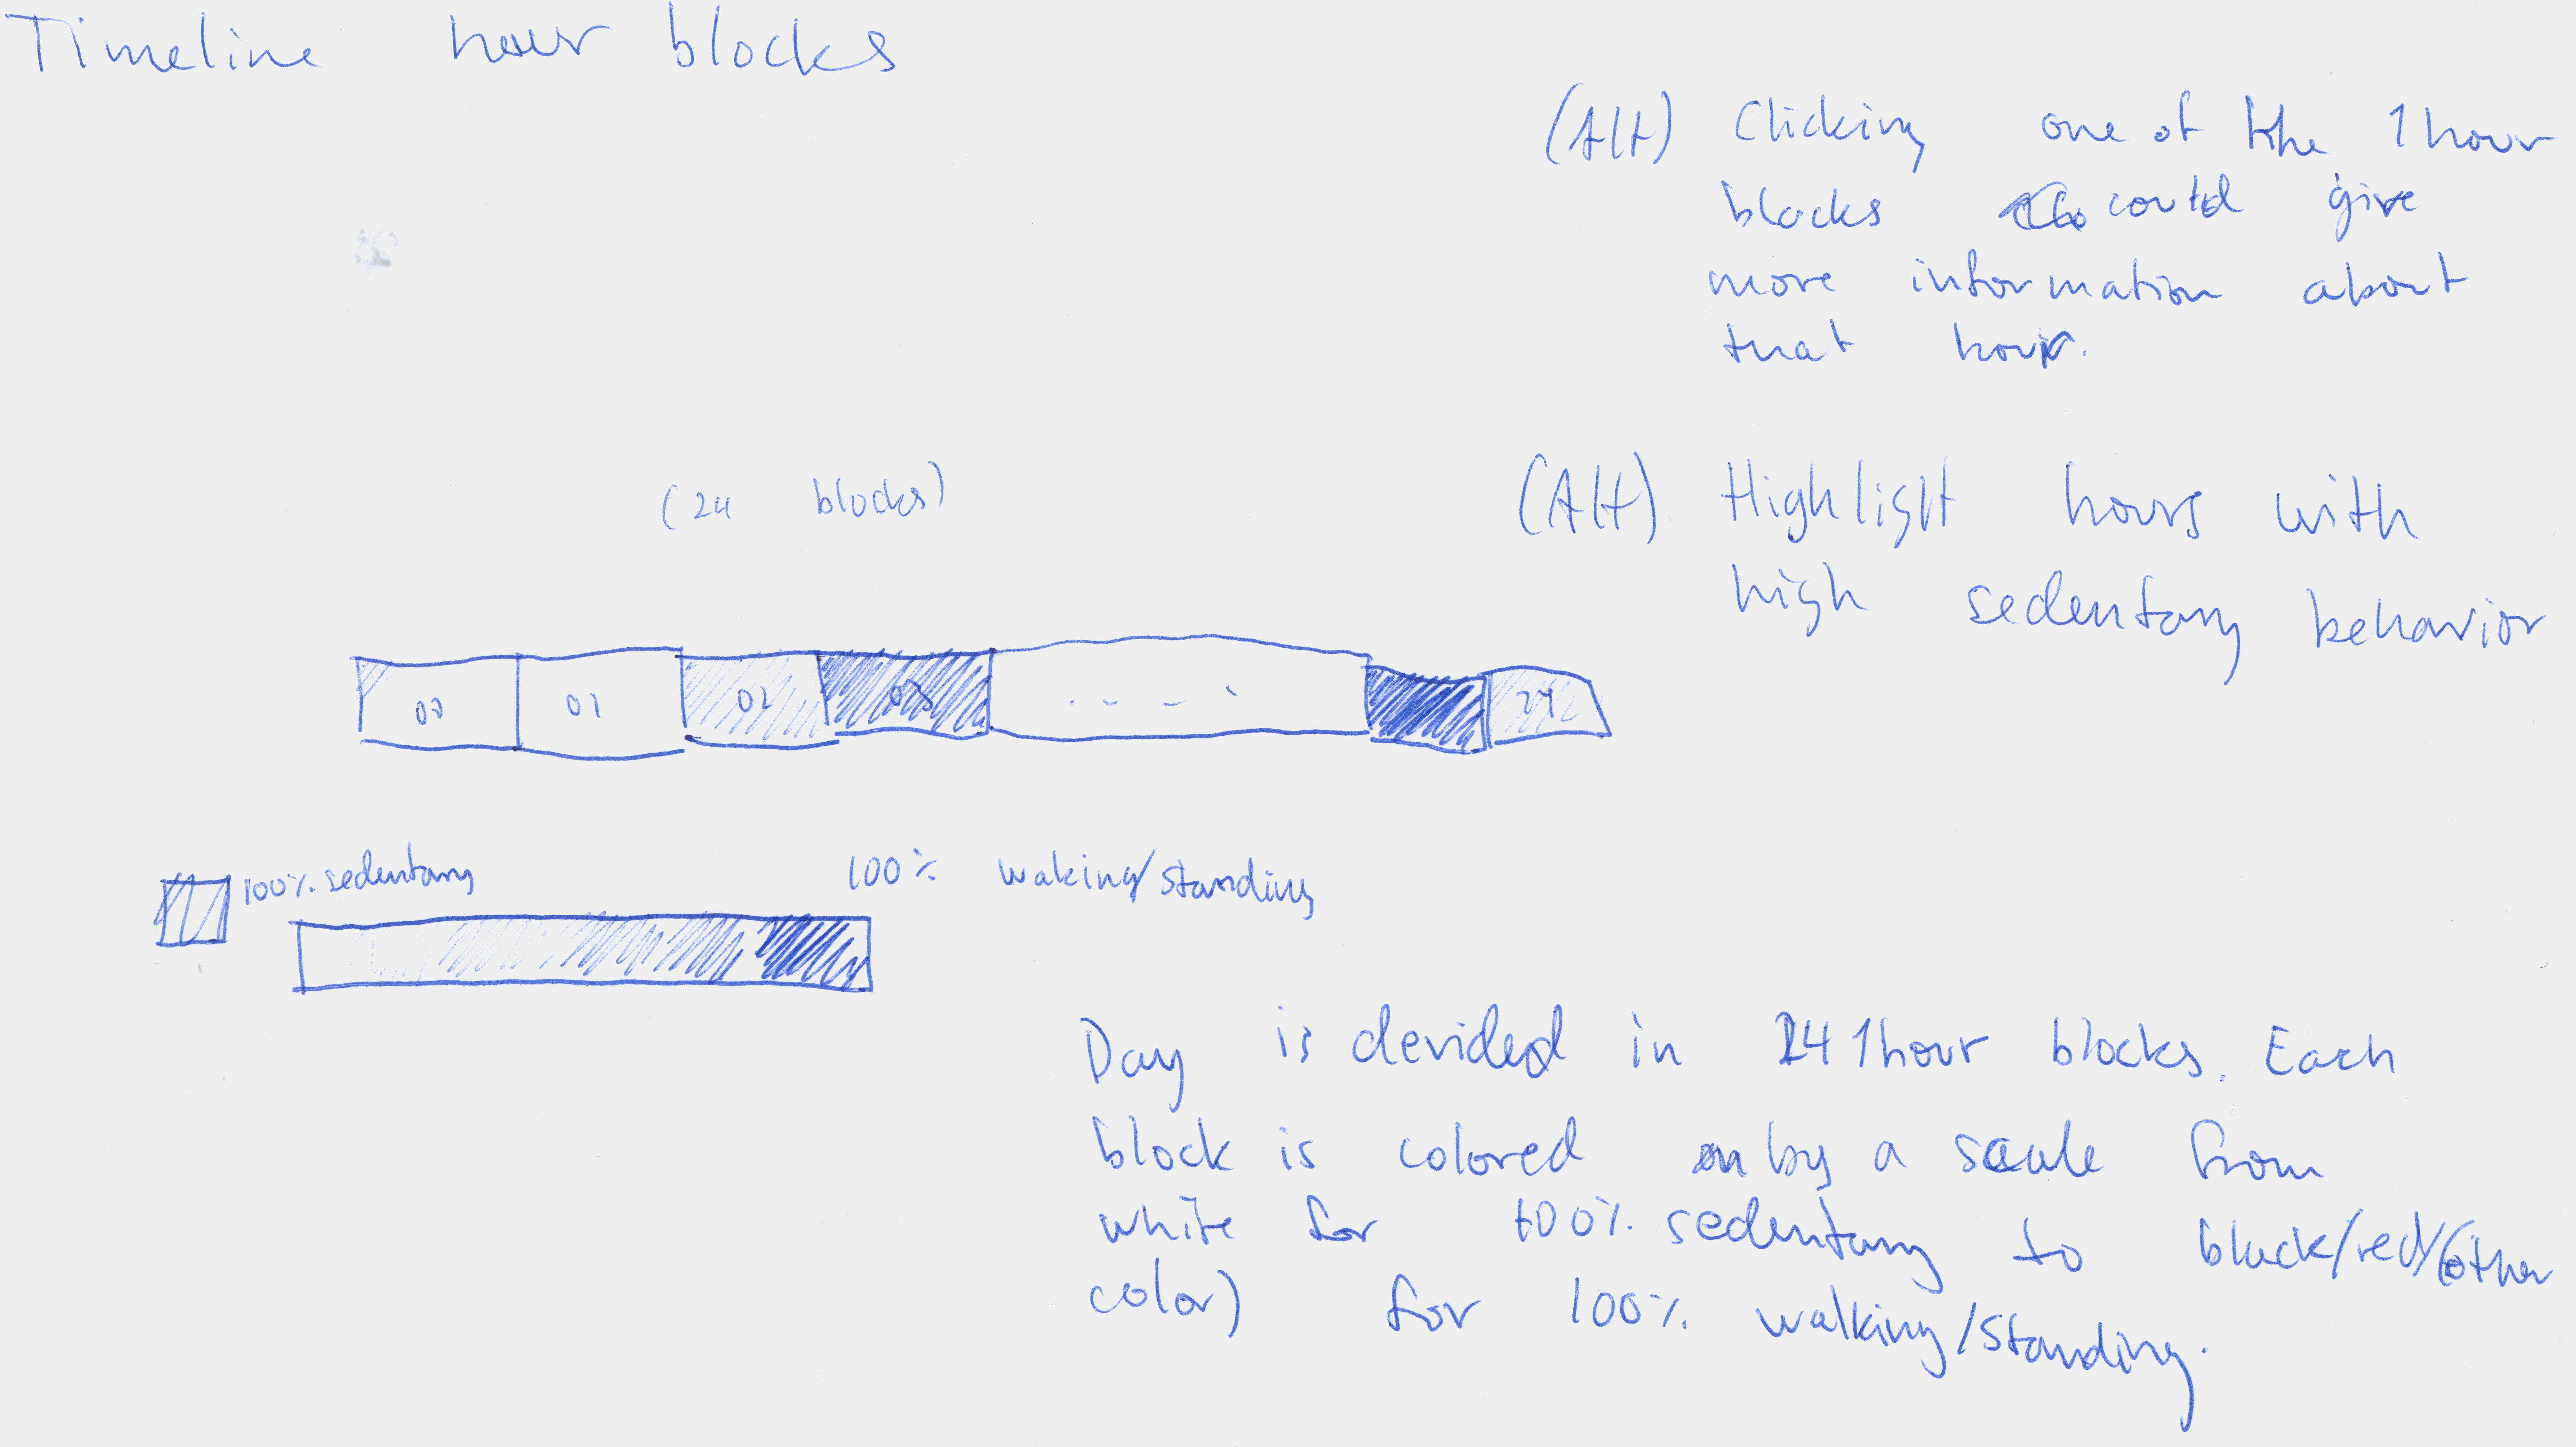
\includegraphics[width=0.7\textwidth]{timelineBlocksSketch.png}
		\caption{\footnotesize Timeline with hour blocks}
		\label{fig:timelineBlocks}
\end{figure}

\subsubsection{Clock}
%Is this part too short now?
A timeline may need some explanation before the user understands it properly. By creating two clocks instead of a long horizontal bar the user can more intuitively understand what the visualization is presenting. Since a clock has only 12 hours, two clocks would need to be drawn. To make it easier to identify day and night, a descriptive background will be added, see figure \ref{fig:clock12}.

\begin{figure}[h!]
	\centering
		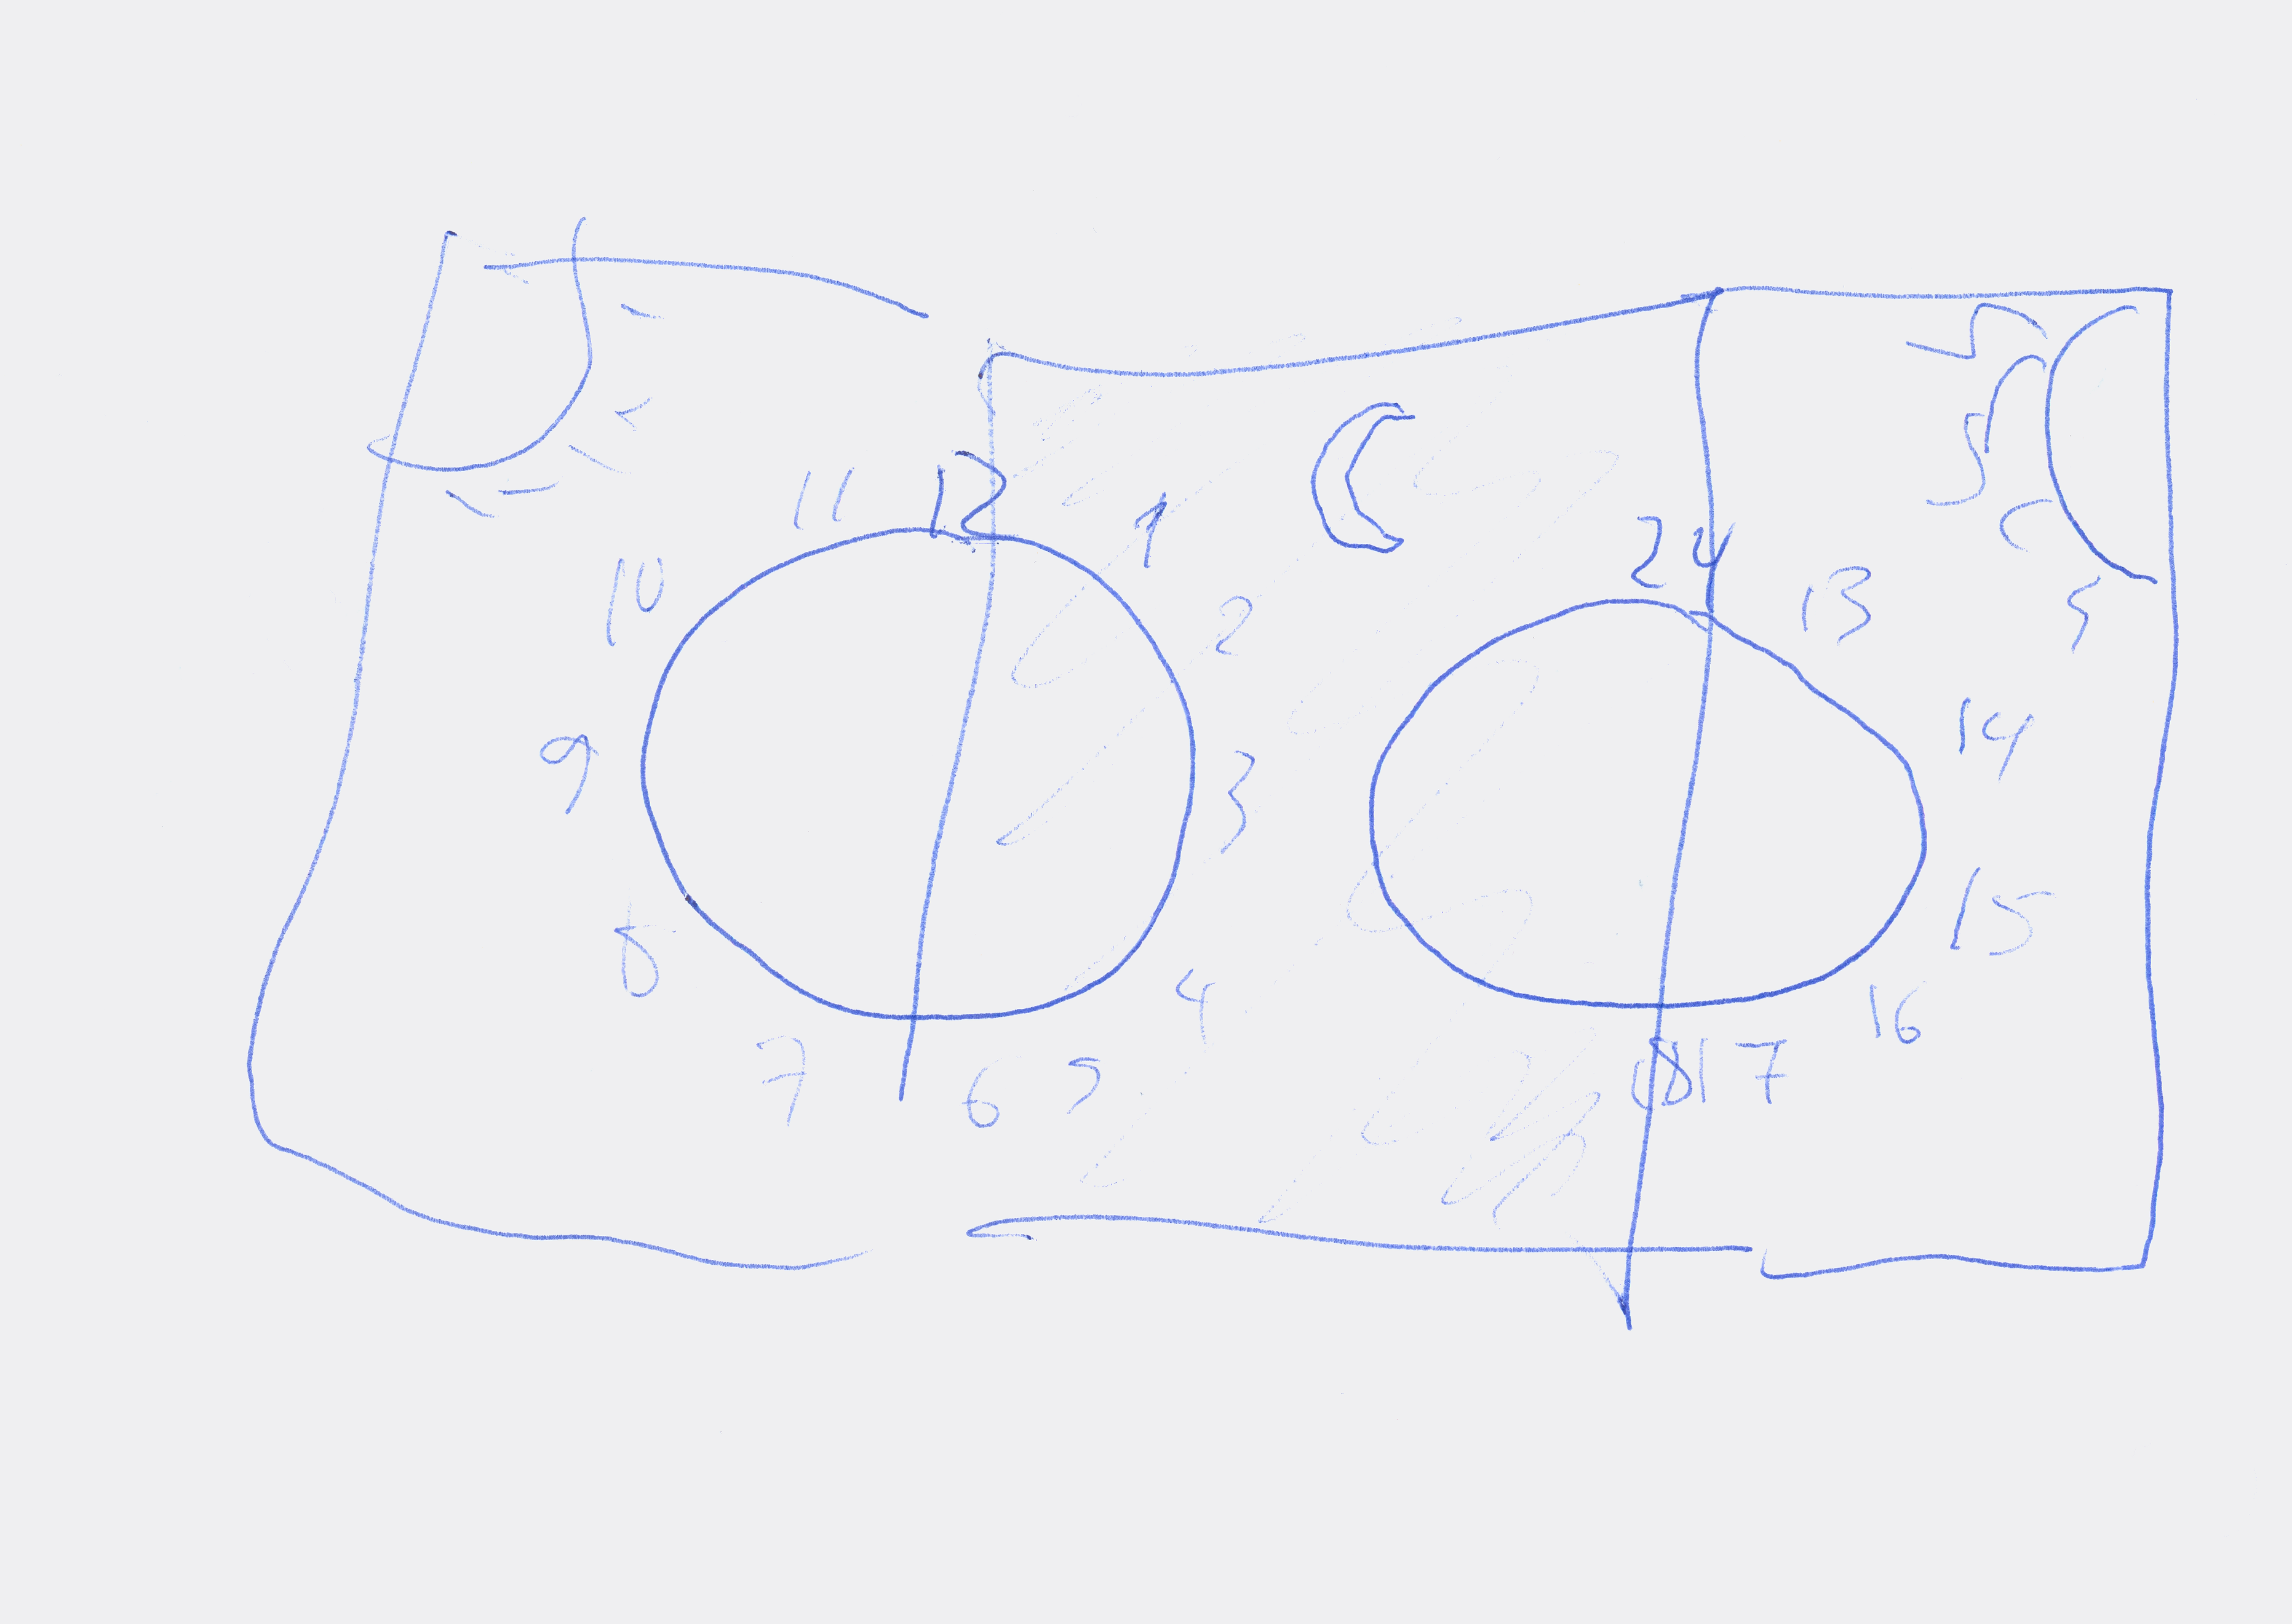
\includegraphics[width=0.7\textwidth]{clock12Sketch.png}
		\caption{\footnotesize Two 12 hour clocks show the activity of the day.}
		\label{fig:clock12}
\end{figure}

Another approach is to use one 24 hour clock, see figure \ref{fig:clock24}. This makes it easier to see the transition between AM and PM, but the users will not be used to seeing a 24 hour clock. This clock will also utilize different background to differentiate between day and night more easily.

\begin{figure}[h!]
	\centering
		
\includegraphics[width=0.5\textwidth]{placeholder.jpg}
		\caption{\footnotesize A single 24 hour clocks show the activity of the day.}
		\label{fig:clock24}
\end{figure}

%Might add a paragraph about highlighting long periods of sedentary behaviour.

\subsection{Week overview}
Getting an overview of the week as a whole can be useful as an introduction. By looking at an overview the user can quickly identify problem days that can then be investigated further. These charts could also be used as the top level of an interactive application. Each day could then be clicked to show either a timeline or pie chart. 

\subsubsection{Day classification}
By calculating the overall activity level and classifying the days into three categories the user can easily see which days he need to be more active and which days the activity level is satisfactory. In our sketch, see figure \ref{fig:smileyWeek} the three different classifications are illustrated by smilies (smiling face for active days, and sad face for inactive days).

\begin{figure}[h!]
	\centering
		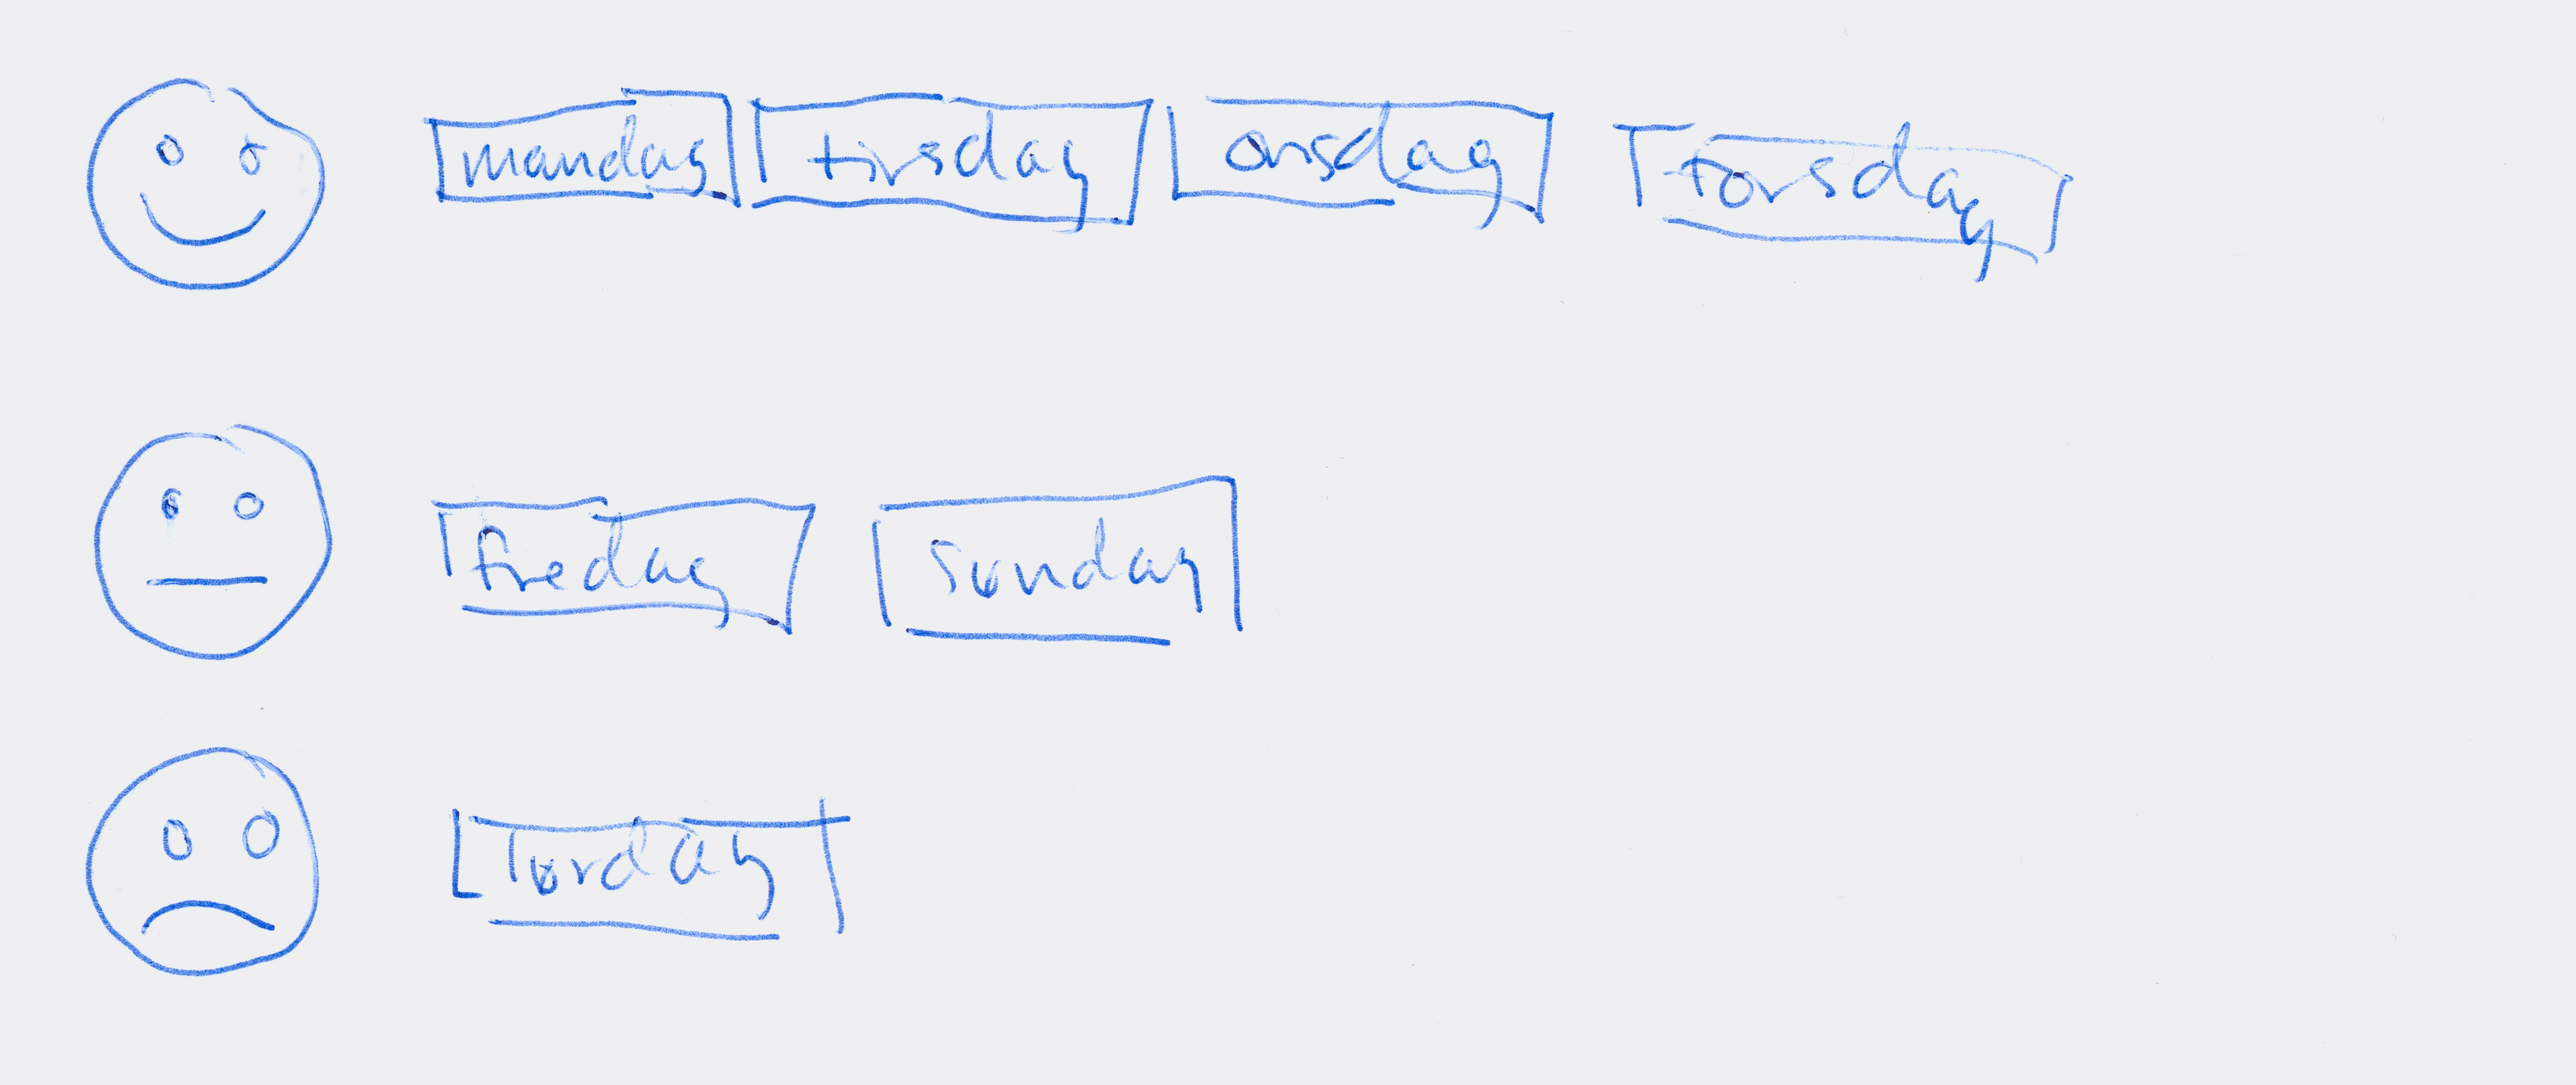
\includegraphics[width=0.7\textwidth]{smileyWeekSketch.png}
		\caption{\footnotesize Week overview with each day classified into one of three categories.}
		\label{fig:smileyWeek}
\end{figure}

A more complex version of the above chart, see figure \ref{fig:detailedWeek} is to show a square for each day, while still using the same classification into sad and happy smilies. Each day square will then contain 24 smaller squares that represent each hour of the day. The small hour square are coloured with a gradient to show the activity level that hour.

\begin{figure}[h!]
	\centering
		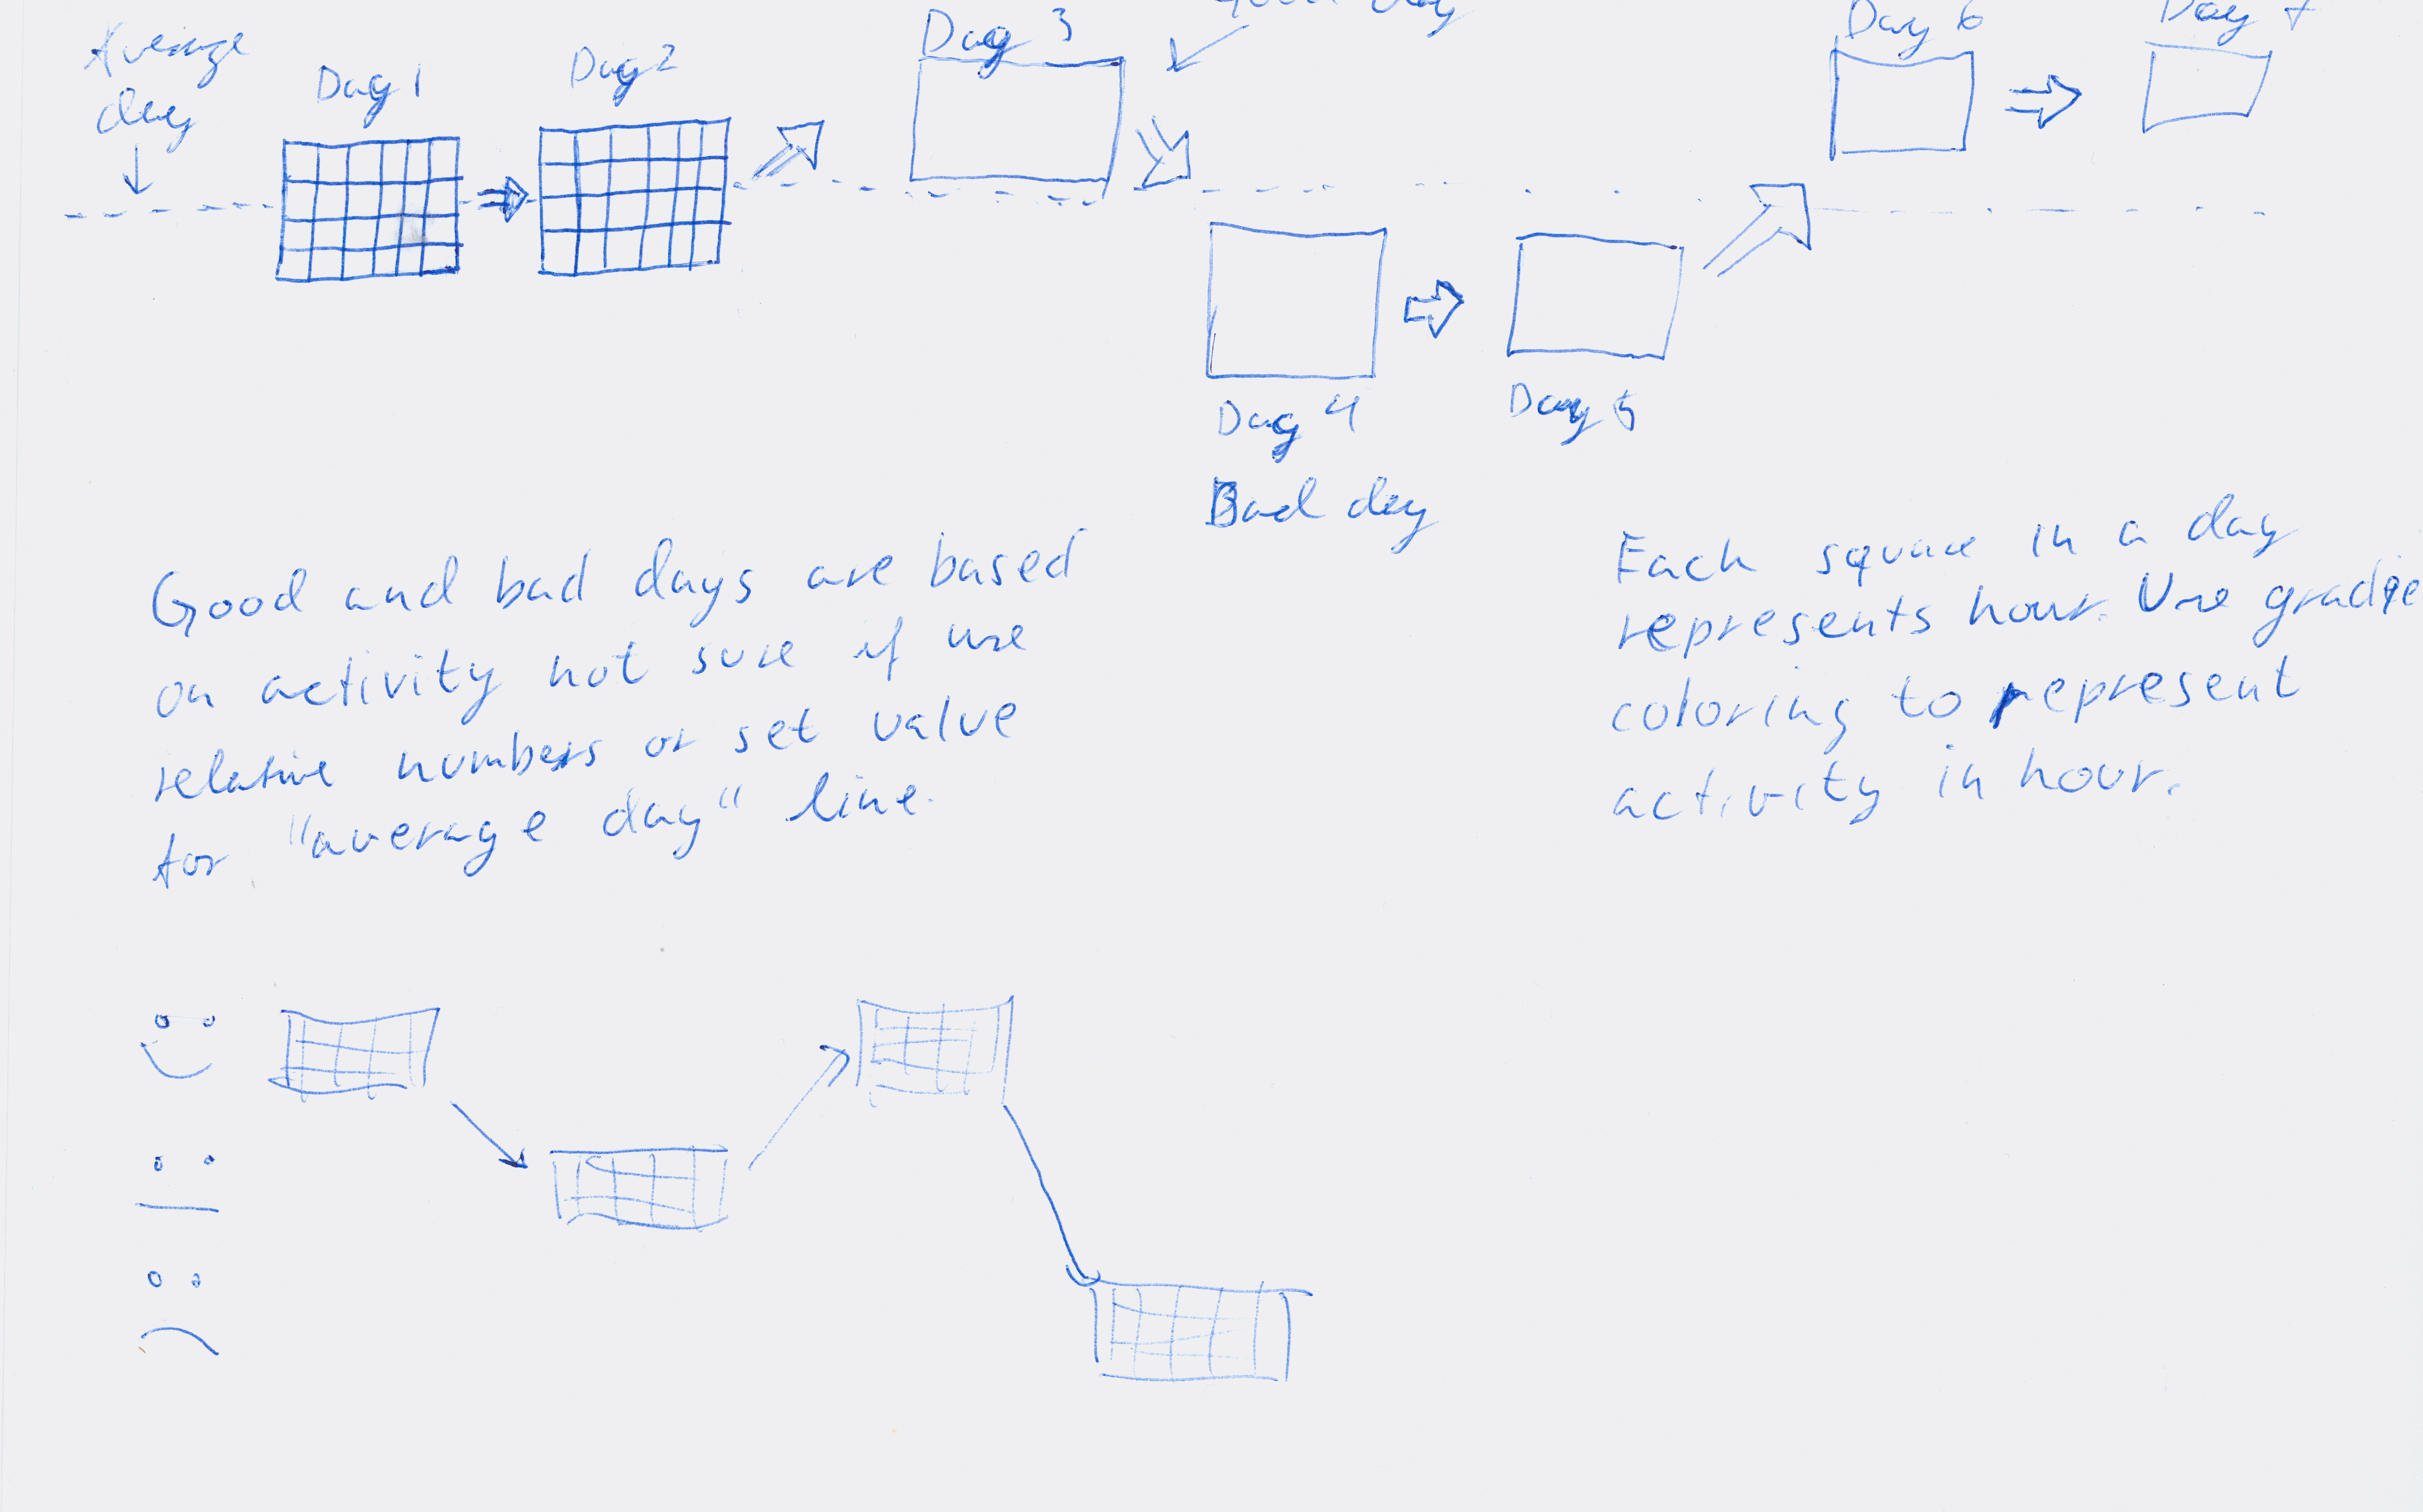
\includegraphics[width=0.6\textwidth]{detailedWeekSketch.png}
		\caption{\footnotesize Some explanation here.}
		\label{fig:detailedWeek}
\end{figure}

With this chart you can get an overview of the week as a whole, and identify what hours of the inactive days had the most sedentary behaviour. 

%This should be moved I guess, or the section should be renamed away from prototype to something like "Graphs" I am not sure.
\section{Hypothesis}
During the initial creation of the graphs %(rename to workshop?) 
we discussed what purpose each graph was designed to serve. A set of hypothesis were created to facilitate our assumptions and allow them to be confirmed or disproved. The graphs are primarily compared to those within the same category as they have been divided to in section \ref{sec:initialGraphs}

\begin{description}
\item[Hypothesis F1:] The stick figures will make the symbolic box chart more intuitive than the pie chart, removing the need for legends.

\item[Hypothesis F2:] The bubble chart is effective at getting the overall distributions of time spent in the different activities.

\item[Hypothesis F3:] The bubble chart makes it easy to identify interval of high sedentary time.

\item[Hypothesis F4:] The pie chart is more likeable then the other fractional charts.

\item[Hypothesis T1:] The blocked timeline makes it easier to identify hours of the day with high sedentary instead of the continuous timeline.

\item[Hypothesis T2:] The extra detail in the continous timeline is useful when going through the patients day.

\item[Hypothesis T3:] Two 12 hour clocks are easier to interpret then a single 24 hour clock.

\item[Hypothesis T4:] It is easier to analyze the day using a timeline than a clock layout.

\item[Hypothesis T5:] The highlighting makes identify periods of high sedentary behaviour easier.

\item[Hypothesis T6:] The switch view function is useful for comparing days quickly ()

\item[Hypothesis T5:] It is easier to analyze the day using a timeline than a clock layout.

\item[Hypothesis W1:] The week is useful for quickly identifying days with high sedentary behaviour.

\item[Hypothesis W2:] The extra information in detailed week is not necessary in a overview setting.

\end{description}



\section{Findings}


\renewcommand*{\bibname}{References}
\bibliographystyle{unsrtnat}
\bibliography{main}

%% Uncomment the following if you have any appendix
% \appendix
% \addtocontents{toc}{%
%  \protect\vspace{1em}% 

%  \protect\noindent \bfseries \appendixtocname\protect\par
%  \protect\vspace{-.5em}%
% }
% \renewcommand{\chaptername}{\appendixname}
%% include below possible appendices (chapters)


\end{document} 
